\chapter{Methodology}
\label{ch:methodology}
The overall process of developing the WebCrowd platform of this work consited of the following steps:
\begin{enumerate}
  \item Theoretical design of the platforms Architecture
  \item Development of a Proof of Concept prototype
  \item Development process of the WebCrowd platform
  \begin{itemize}
    \item Implementation of \acs{API} and web interface
    \item Usage of generic job and task entities to support any kind of custom job
    \item Add WebAssembly Support for multiple programming languages
    \item Implement support for various output datatypes (primitiv datatypes, lists, files in binary format)
  \end{itemize}
  \item Deployment of the web application
  \begin{itemize}
    \item Dockerize all components of the WebCrowd platform
    \item Host the project on a cloud services
    \item Implement users and user roles
    \item Implement security measures through authentication \& authorization
  \end{itemize}
  \item Enhance robustness of the platform
  \begin{itemize}
    \item Implement system recovery measures and persistence of critical data
    \item Adjust scheduling algorithem to ensure the completion of jobs with unreliable workers
    \item Eliminate bugs through testing the application
  \end{itemize}
  \item Implement a benchmark job
  \item Benchmark the platform with multiple experiments 
\end{enumerate}
This chapter enumerates and describes all the technologies, frameworks, and tools utilized in the development of the volunteer computing platform, along with the reasoning for their selection. Each section provides a detailed explanation of these components, establishing a foundation for the following chapter, \ref{ch:implementation} Implementation. Additionally, all entities are listed and described in section \ref{sec:methodology:entities} to define the specific terms used in the subsequent chapters.

\section{Entities}
\label{sec:methodology:entities}
This section describes all entities and establishes the terms used to describe the processes in this work.

\subsection{Job}
\label{subsec:methodology:entities:job}
The Job entity represents a problem to be processed or solved using the platform. The platform is designed to handle multiple Jobs while each Job is a unique object. The State of a Job can have one of the following values:
\begin{itemize}
  \item PENDING
  \item ACTIVE
  \item RUNNING
  \item STOPPED
  \item DONE
\end{itemize}
Figure \ref{fig:methodology:job-task} illustrates the \ac{UML} class diagram for the Job entity on the left side, lisitng all important attributes and methods of a Job. The language attribute defines the programming langugae of the source code that has been compiled to a WebAssembly binary file.
\begin{figure}[htbp]
  \centering
  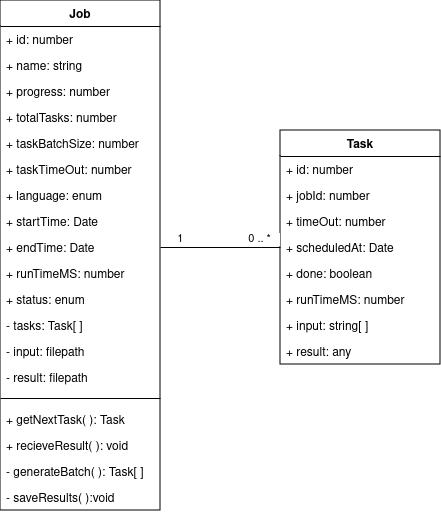
\includegraphics[width=0.75\textwidth]{gfx/figures/Job-Task.png}
  \caption{\ac{UML} Class Diagram: Job \& Task}
  \label{fig:methodology:job-task}
\end{figure}

\subsection{Task}
\label{subsec:methodology:entities:task}
Each Job is divided into multiple equally sized Tasks. These Tasks are distributed to the worker nodes of the platform. Tasks are unique objects, each holding the specific input parameters that describe the particular portion of the Job to which the Task is assigned. Figure \ref{fig:methodology:job-task} displays the \ac{UML} class diagram for the Task entity on the right side. The relationship between Job and Task entities is defined as One-to-Many, meaning a Job can consist of multiple Tasks, but each Task is always assigned to a single Job.

\subsubsection{Batch}
\label{ssubsec:methodology:entities:task:batch}
A Batch is defined to be a subset of Tasks, wich are all assigned to the same Job.

\subsection{Client}
\label{subsec:methodology:entities:client}
A Client represents a node that accesses the platform. The actions a Client can perform are determined by the User Role assigned to its User. This User Role can have one of the following values:
\begin{itemize}
  \item User
  \item Admin
\end{itemize}
Figure \ref{fig:methodology:client} displays the \ac{UML} class diagram for the User entity at the top of the illustration.
\begin{figure}[htbp]
  \centering
  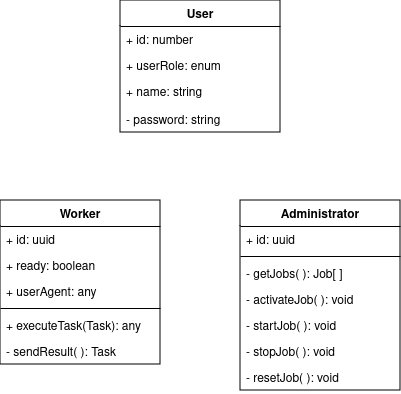
\includegraphics[width=0.75\textwidth]{gfx/figures/Client.png}
  \caption{\ac{UML} Class Diagram: User - Worker \& Administrator}
  \label{fig:methodology:client}
\end{figure}

\subsubsection{Worker}
\label{ssubsec:methodology:entities:client:worker}
Workers are Clients that voluntarily donate their computing power to support an active Job. Therfore they receive Tasks from the current Batch sent by the Server (\ref{subsec:methodology:entities:Server}), compute these Tasks, and return the corresponding results back to the Server. Figure \ref{fig:methodology:client} presents the \ac{UML} class diagram of the Worker entity on the left side, listing all relevant attributes and methods. As Workers connect to the Server via web browsers, the browser's User Agent is utilized to individually characterize each worker. A browser User Agent can provide information about the Client's hardware resources and operating system.

\subsubsection{Administrator}
\label{ssubsec:methodology:entities:client:admin}
An Administrator Client can perform the same actions as a Worker, but also has additional capabilities. Only Administrators have the ability to set or change the state of Jobs and to oversee the progress of all Jobs. Figure \ref{fig:methodology:client} illustrates the \ac{UML} class diagram of the Administrator entity on the right side.

\subsection{Server}
\label{subsec:methodology:entities:Server}
The Server is used as the central component to maintain the network. Each Client intending to connect to the network must establish a connection with the Server.

Additionally the Server is responsible for scheduling and distributing the Tasks to all Workers. It also persistently stores each Job along with all results of its corresponding Tasks.

\section{Database}
An object-relational database system was identified to fulfill the platform's requirements, as these systems typically offer high performance capabilities and the entities described in the previous sections can be represented with an object-relational database schema.

PostgreSQL is an open source object-relational database system that has been actively developed for more than 35 years \cite{methodology:db}. Therefore it has gained a strong reputation for reliability, feature robustness, and performance \cite{methodology:db}, hence PostgreSQL was selected as the database management system for this implementation.

\section{WebAssembly - TODO}
\label{sec:methodology:wasm}
WebAssembly is a key technology in this proposed system, offering several advantages for distributed computing. It provides near-native performance, platform independence, and potential multi-threading capabilities. WebAssembly allows to compile code written in languages such as C, C++, and Rust to a binary format that can be executed in web browsers, enabling efficient computation on diverse client devices.

(TODO: List / tabel of web browsers that support wasm socket and)

WebAssembly (Wasm) is a low-level binary instruction format designed to serve as a compilation target for high-level languages, enabling near-native performance execution in web browsers. It employs a stack-based virtual machine architecture, operates in a memory-safe sandboxed environment, and interfaces with JavaScript through a defined API. The compiled Wasm modules execute at machine code speed, making it particularly effective for computationally intensive tasks like image processing, game engines, or cryptographic operations, while maintaining the web's security model.

\cite{methodology:wasm, methodology:wasmdocu, relatedwork:wasmedgecomputing}

\subsection{emscriptren for C and C++}
\label{subsec:methodology:wasm:cpp}
compiler from C \& C++ to .wasm with .js Gluecode (setup wasm environment) \cite{methodology:emcc}
\subsection{Go}
\label{subsec:methodology:wasm:go}
compiler from Go to .wasm, offically from Go \cite{methodology:go}
\subsection{Pyodie for Python}
\label{subsec:methodology:wasm:python}
"Pyodide is a port of CPython to WebAssembly/Emscripten". \cite{methodology:pyodie}

\section{WebSokets - TODO}
\label{sec:methodology:websokets}
WebSockets play a crucial role in this system's communication infrastructure. Unlike traditional HTTP requests, WebSockets enable faster, bidirectional communication between clients and servers. This real-time capability is essential for efficient task distribution, progress monitoring, and result collection in the distributed computing platform.

WebSocket is a bidirectional, full-duplex communication protocol operating over a single TCP connection, defined in RFC 6455. Unlike traditional HTTP request-response patterns, WebSocket enables persistent connections between client and server, allowing real-time data transmission in both directions with minimal overhead after the initial handshake. The protocol utilizes the ws:// or wss:// (secure) URI scheme and efficiently handles scenarios requiring live updates such as financial trading platforms, multiplayer games, or chat applications, with significantly reduced latency compared to polling mechanisms.

\cite{methodology:websockets1, methodology:websockets2, methodology:websockets3}

\section{WebWorker - TODO}
\label{sec:methodology:webworker}
Web Workers are employed to enhance the performance and responsiveness of client-side computations. By executing computationally intensive tasks in separate threads, Web Workers prevent blocking the main thread responsible for the user interface and other critical browser functions. This approach allows our system to utilize client resources more effectively while maintaining a smooth user experience.

WebWorkers are a JavaScript API that enables concurrent execution of scripts in background threads separate from the main browser UI thread. They operate in an isolated context, communicating with the main thread via a message-passing interface (postMessage), and cannot directly manipulate the DOM. This implementation of parallel processing prevents CPU-intensive tasks from blocking the user interface, making them optimal for computationally heavy operations such as data processing, complex calculations, or cryptographic operations. WebWorkers maintain browser performance by adhering to a strict same-origin policy and limited access to core JavaScript features.

\cite{methodology:webworkers}

\section{Frameworks}
\label{sec:methodology:frameworks}
This section introduces the frameworks selected for the development of the web application. The following criteria were used to guide the selection of a suitable framework for the backend as well as the frontend:
\begin{itemize}
    \item The framework is well-tested and provides a stable \ac{LTS} version.
    \item The framework is popular among web developers.
    \item I am familiar with the programming language.
\end{itemize}

\subsection{Backend}
\label{subsec:methodology:frameworks:backend}
It was crucial for the backend framework to be popular among web developers. Working with a popular framework improves the development process by ensuring the availability of extensive educational and support resources online. Additionally, a widely used framework increases the likelihood that the platform can be maintained or further extended by other programmers.
\begin{figure}[htbp]
 \centering
 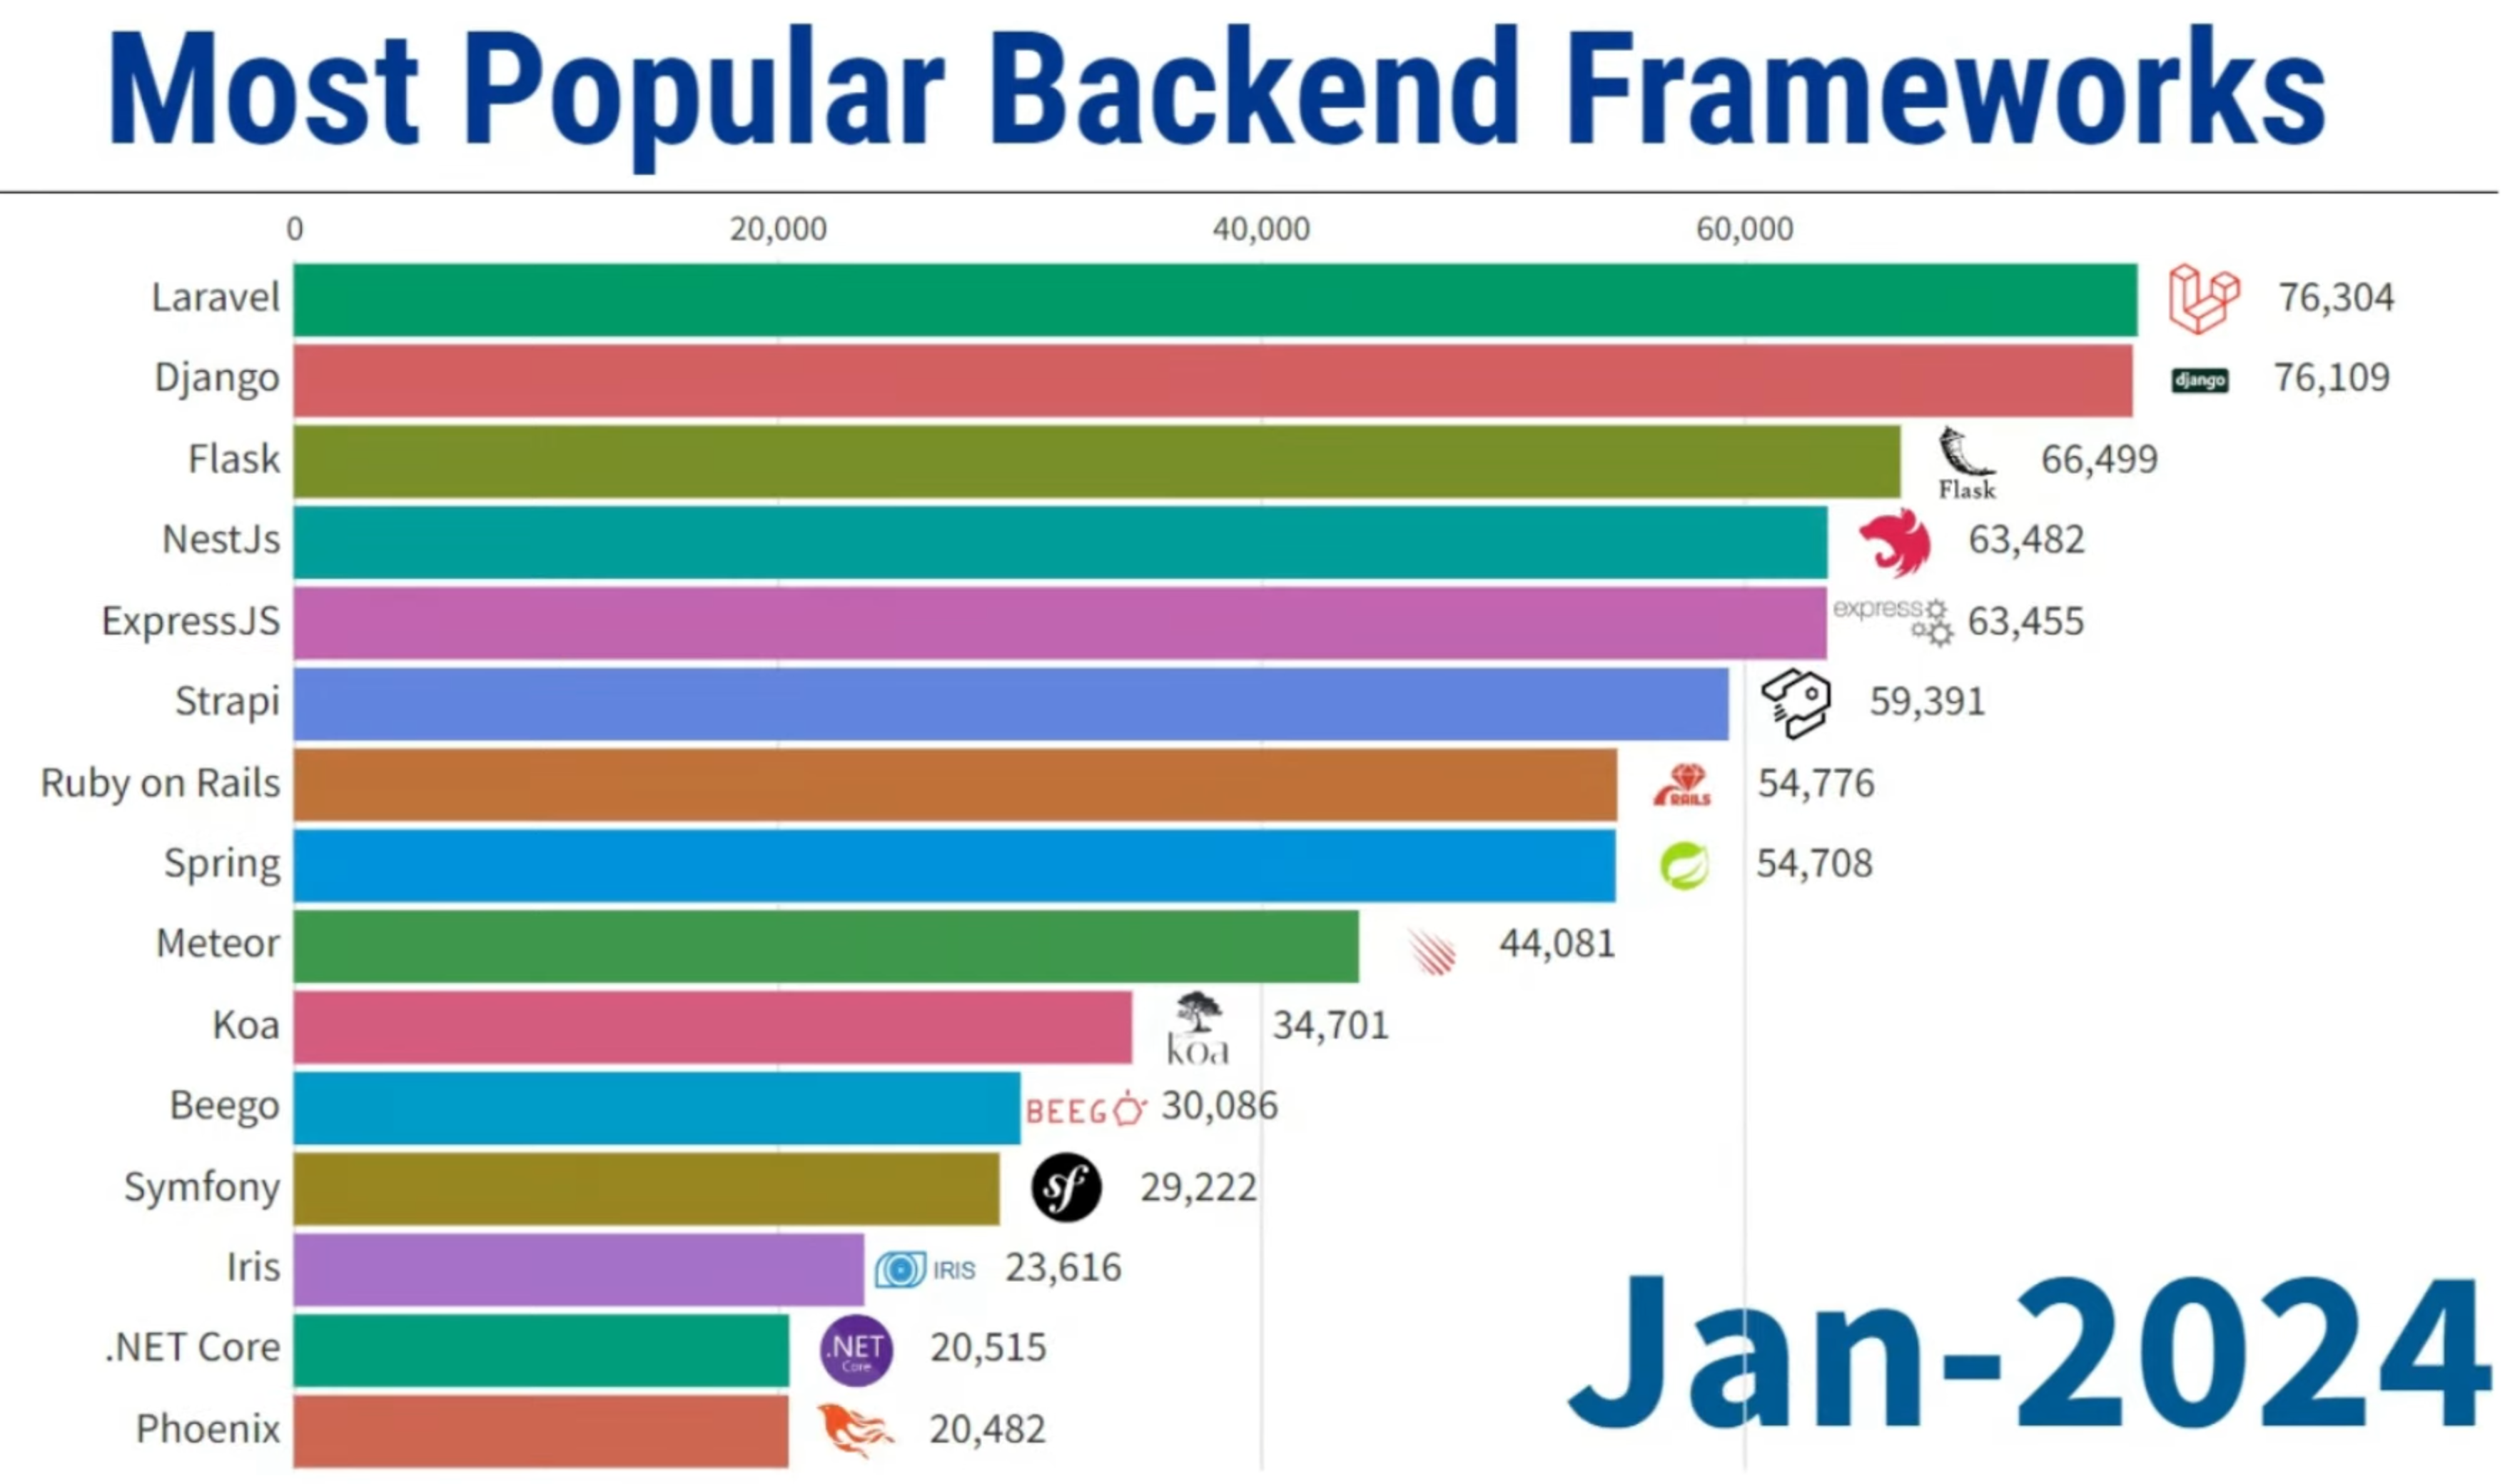
\includegraphics[width=0.95\textwidth]{gfx/figures/Popular_BE.png}
 \caption{Most Popular Backend Frameworks (Jan 2024) by GitHub Stars \cite{backend:popularity}}
 \label{fig:methodology:popularBE}
\end{figure}
The 15 most popular backend frameworks of January 2024 are displayed in figure \ref{fig:methodology:popularBE}. The popularity for each framework of this list is calculated by the number of GitHub Stars from repositories listed in a GitHub Archive \cite{backend:popularity}. The selection options of the backend framework where based on this popularity list. 
\begin{figure}[htbp]
  \myfloatalign
  \subfloat[Requests/Second (2024-06-25) \cite{backend:benchmark1}]{
     \label{fig:methodology:benchmark1BE}
     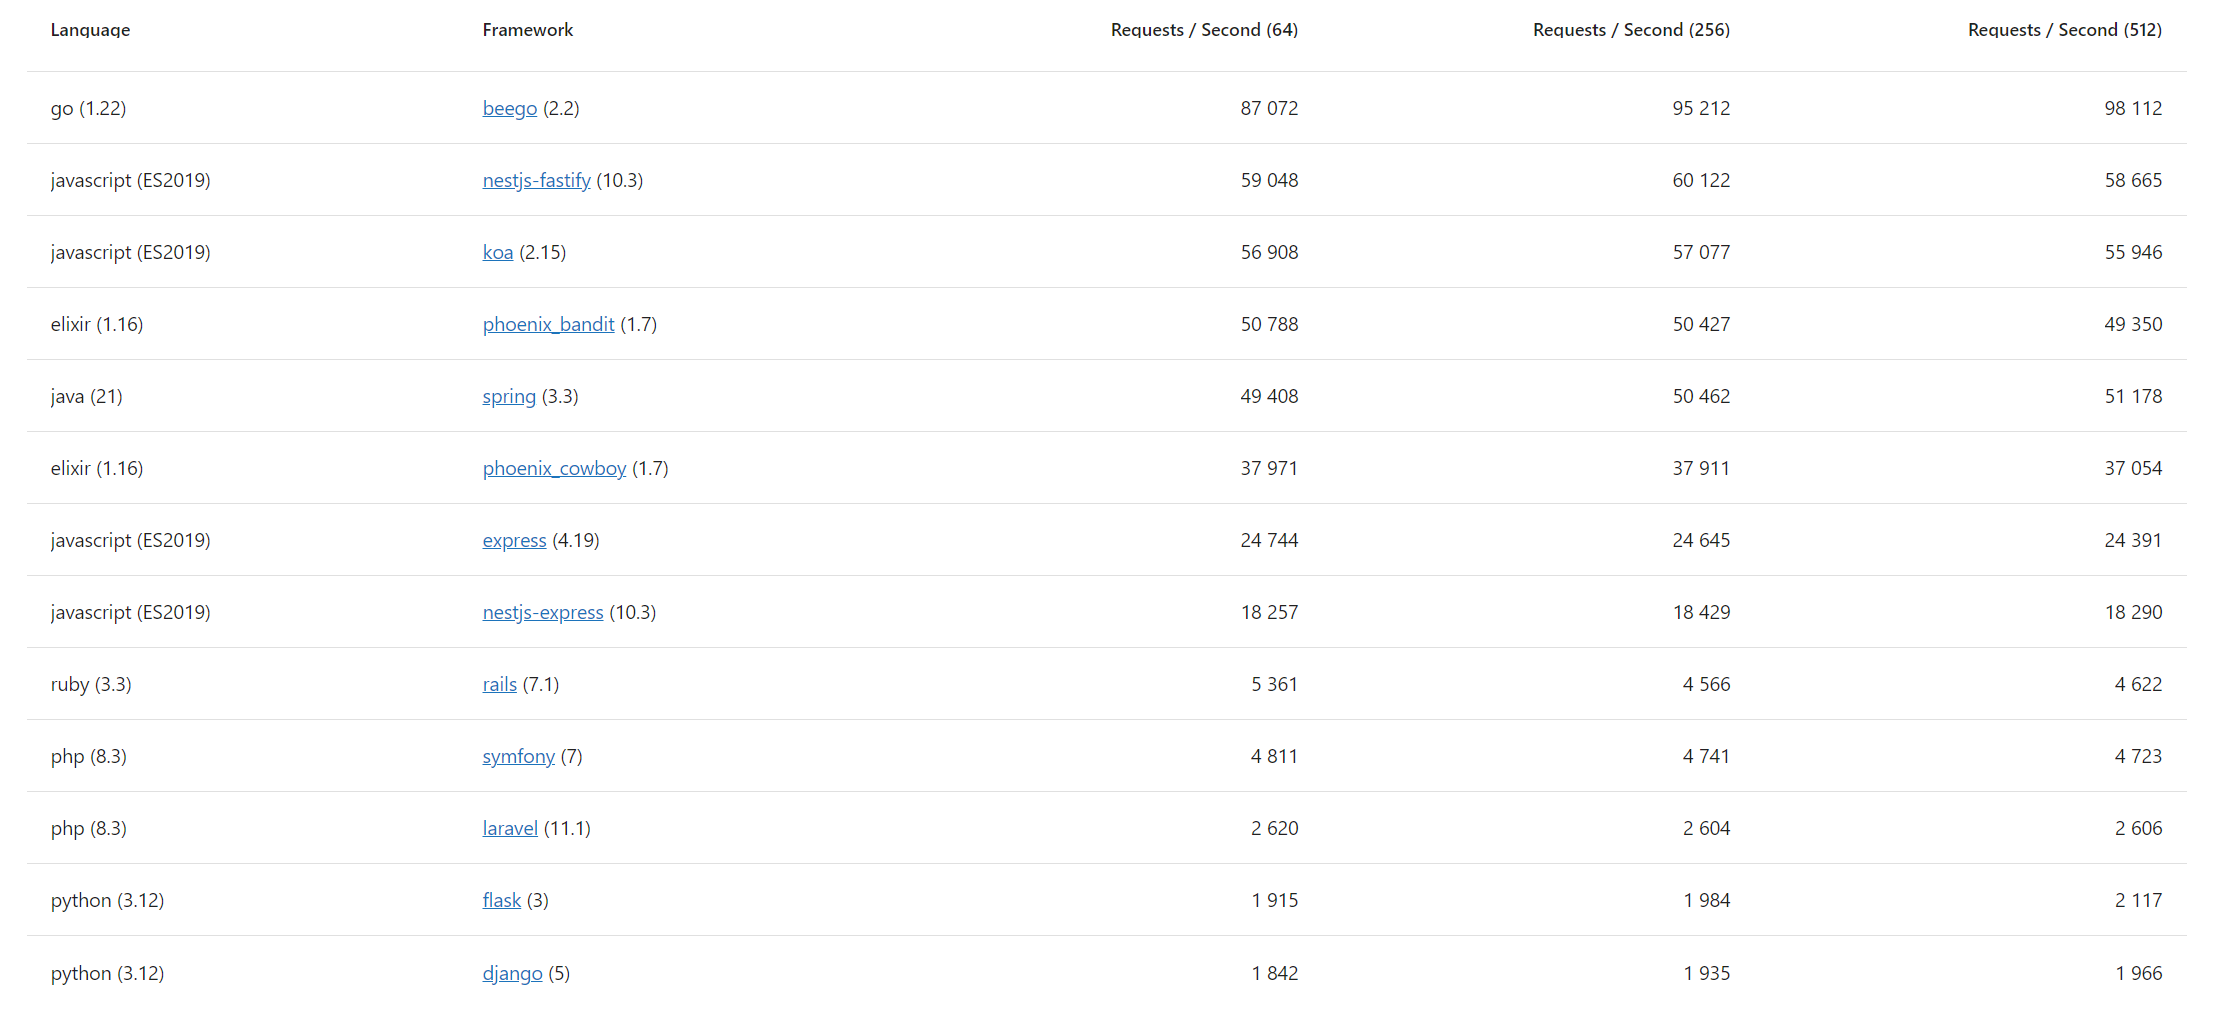
\includegraphics[width=.75\linewidth]{gfx/figures/Benchmark1_BE.png}
   }
   \caption{Most Popular Backend Frameworks from Figure \ref{fig:methodology:popularBE} ranked by Performance.}
   \label{fig:methodology:benchmarkBE}
\end{figure}

\begin{figure}[htbp] \ContinuedFloat
  \myfloatalign
  \subfloat[Best fortunes responses per second (2023-10-17) \cite{backend:benchmark2}]{
    \label{fig:methodology:benchmark2BE}
    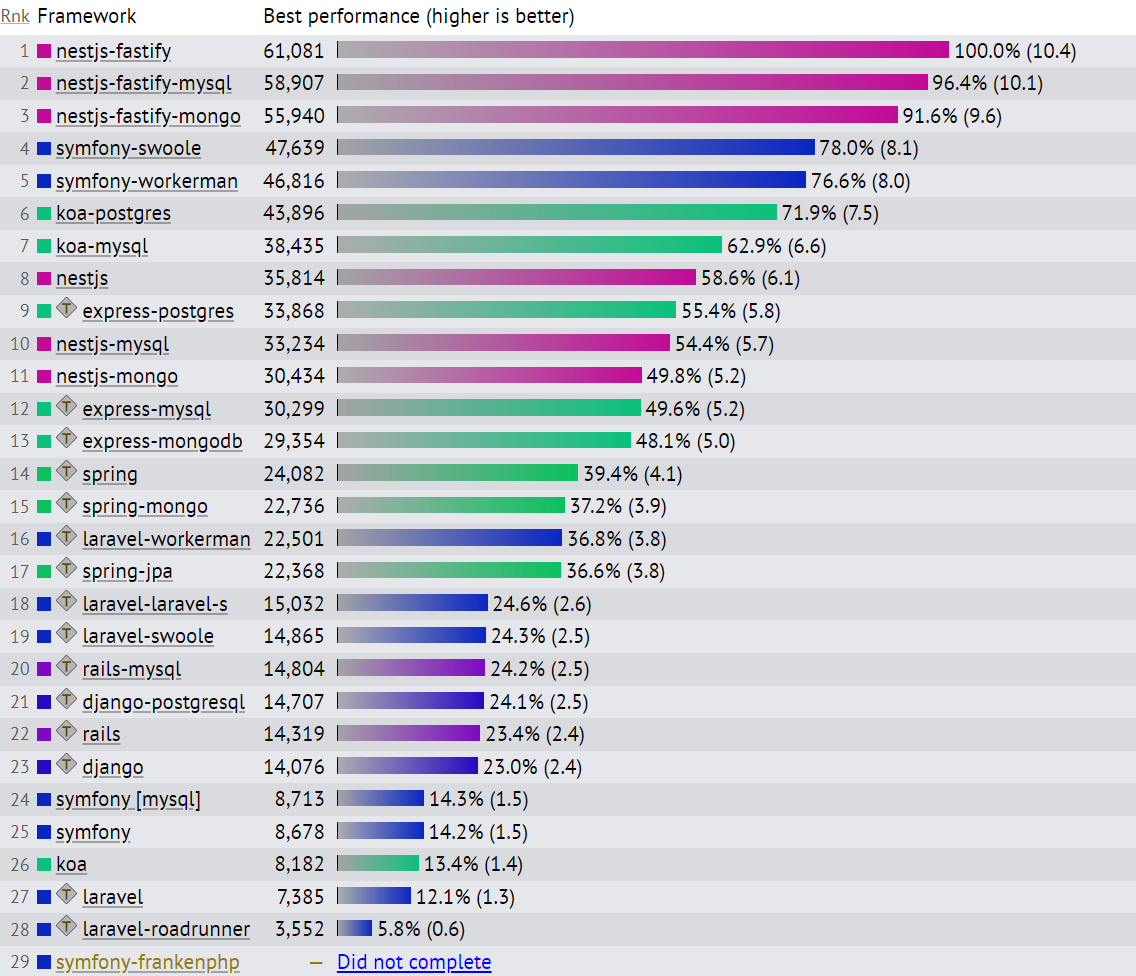
\includegraphics[width=.95\linewidth]{gfx/figures/Benchmark2_BE.png}
  }
\caption{Most Popular Backend Frameworks from Figure \ref{fig:methodology:popularBE} ranked by Performance.}
\label{fig:methodology:benchmarkBE}
\end{figure}
In addition to the previously stated criteria, the selected backend framework needed to meet specific performance requirements. It was essential for the framework to efficiently handle multiple connected clients with minimal latency. Furthermore, the framework's internal computation speed was critical, particularly for preparing input arguments for each task and managing task scheduling across all clients. The goal was to reduce overhead as much as possible to ensure high performance.

To identify a high-performance framework, the most popular backend frameworks listed in Figure \ref{fig:methodology:popularBE} were compared using two different benchmarks. The results of these benchmarks are presented in Figure \ref{fig:methodology:benchmarkBE}, where the frameworks are ranked from top to bottom based on their performance in both benchmarks. It is important to note that some frameworks from the list in Figure \ref{fig:methodology:popularBE} could not be found in these specific benchmarks. Both benchmark sources simulated numerous clients sending requests to each backend and measuring the number of successful responses per second in order to determine the performance \cite{backend:benchmark1, backend:benchmark2}.

Finally, NestJS \cite{methodology:nestjs} with Fastify was selected as the backend framework. It performed exceptionally well in both benchmarks shown in Figure \ref{fig:methodology:benchmarkBE} and is also a popular choice among developers.

\subsection{Frontend}
\label{subsec:methodology:frameworks:frontend}
The criteria stated in \ref{sec:methodology:frameworks} also applied for the selection of a framework for the frontend. Figure \ref{fig:methodology:popularFE} shows the 36 most used frameworks among web developers in July 2024 \cite{frontend:popularity}. This statistic has been collected by Stack Overflow and is the result of a survey. In this survey web developers have been asked which web frameworks and web technologies they had been working with in the past year, and which do they want to work in over the next year \cite{frontend:popularity}. The two must popular options are, by far, Node.js and React with each around 40\% of votes. While Node.js is mainly used for backend development React is a JavaScript library used for frontend development. This is qualifying React as the choice of technology for the frontend development. Ranking fourth in figure \ref{sec:methodology:frameworks} is Next.js with 17.9\% of votes. Next.js is a web framework based on React \cite{methodology:nextjs} and according to the survey the most popular React web framework in the year 2024. Therfore Next.js was selected as the framework for frontend development.
\begin{figure}[htbp]
  \centering
  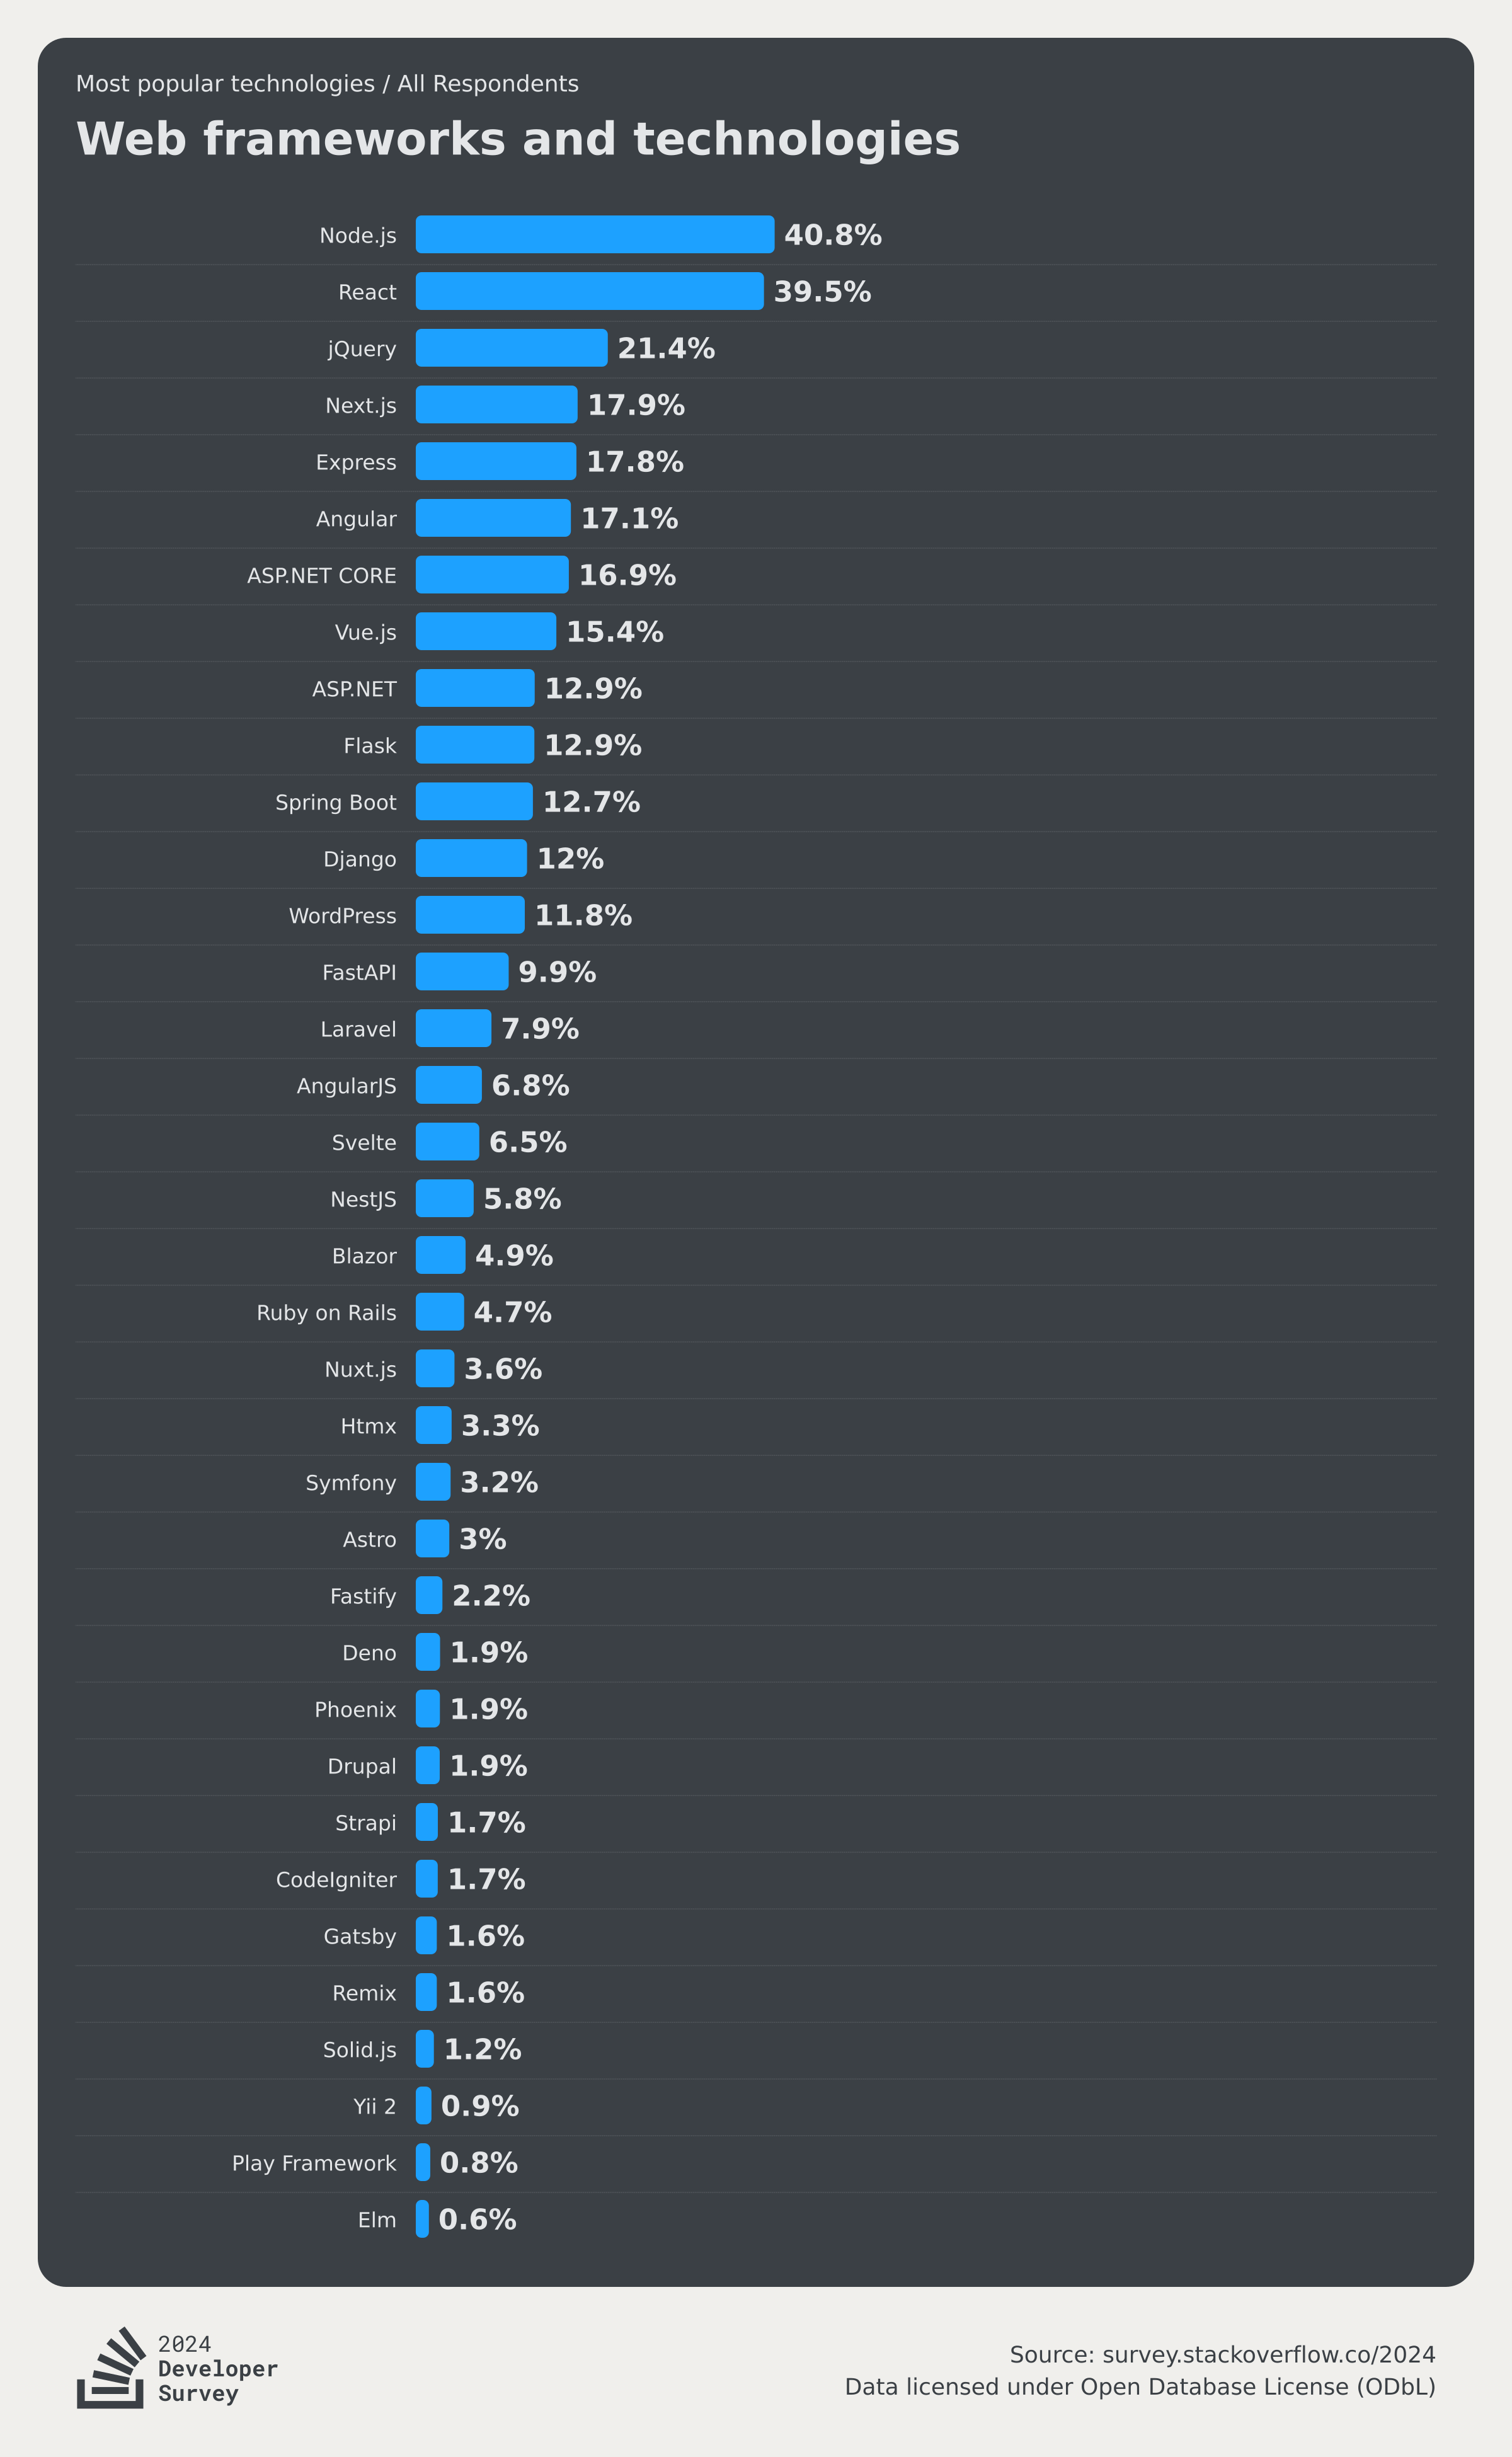
\includegraphics[width=0.95\textwidth]{gfx/figures/FrameworkSurvey2024.png}
  \caption{Most Used Web Frameworks and technologies in 2024 (Developer Survey from Stack Overflow) \cite{frontend:popularity}}
  \label{fig:methodology:popularFE}
\end{figure}

\section{Benchmark: Visualizing the Mandelbrot set}
\label{sec:methodology:benchmark}
To benchmark the platform's performance, a computationally intensive Job is implemented for the platform and executed across multiple connected Workers. The total execution time is compared to the execution time of the same Job on a single machine with native source code. The visualization of the Mandelbrot set represents all characteristics previously described in section \ref{sec:background:theory}, making it suitable as a Job for this benchmark.
\begin{figure}[htbp]
  \centering
  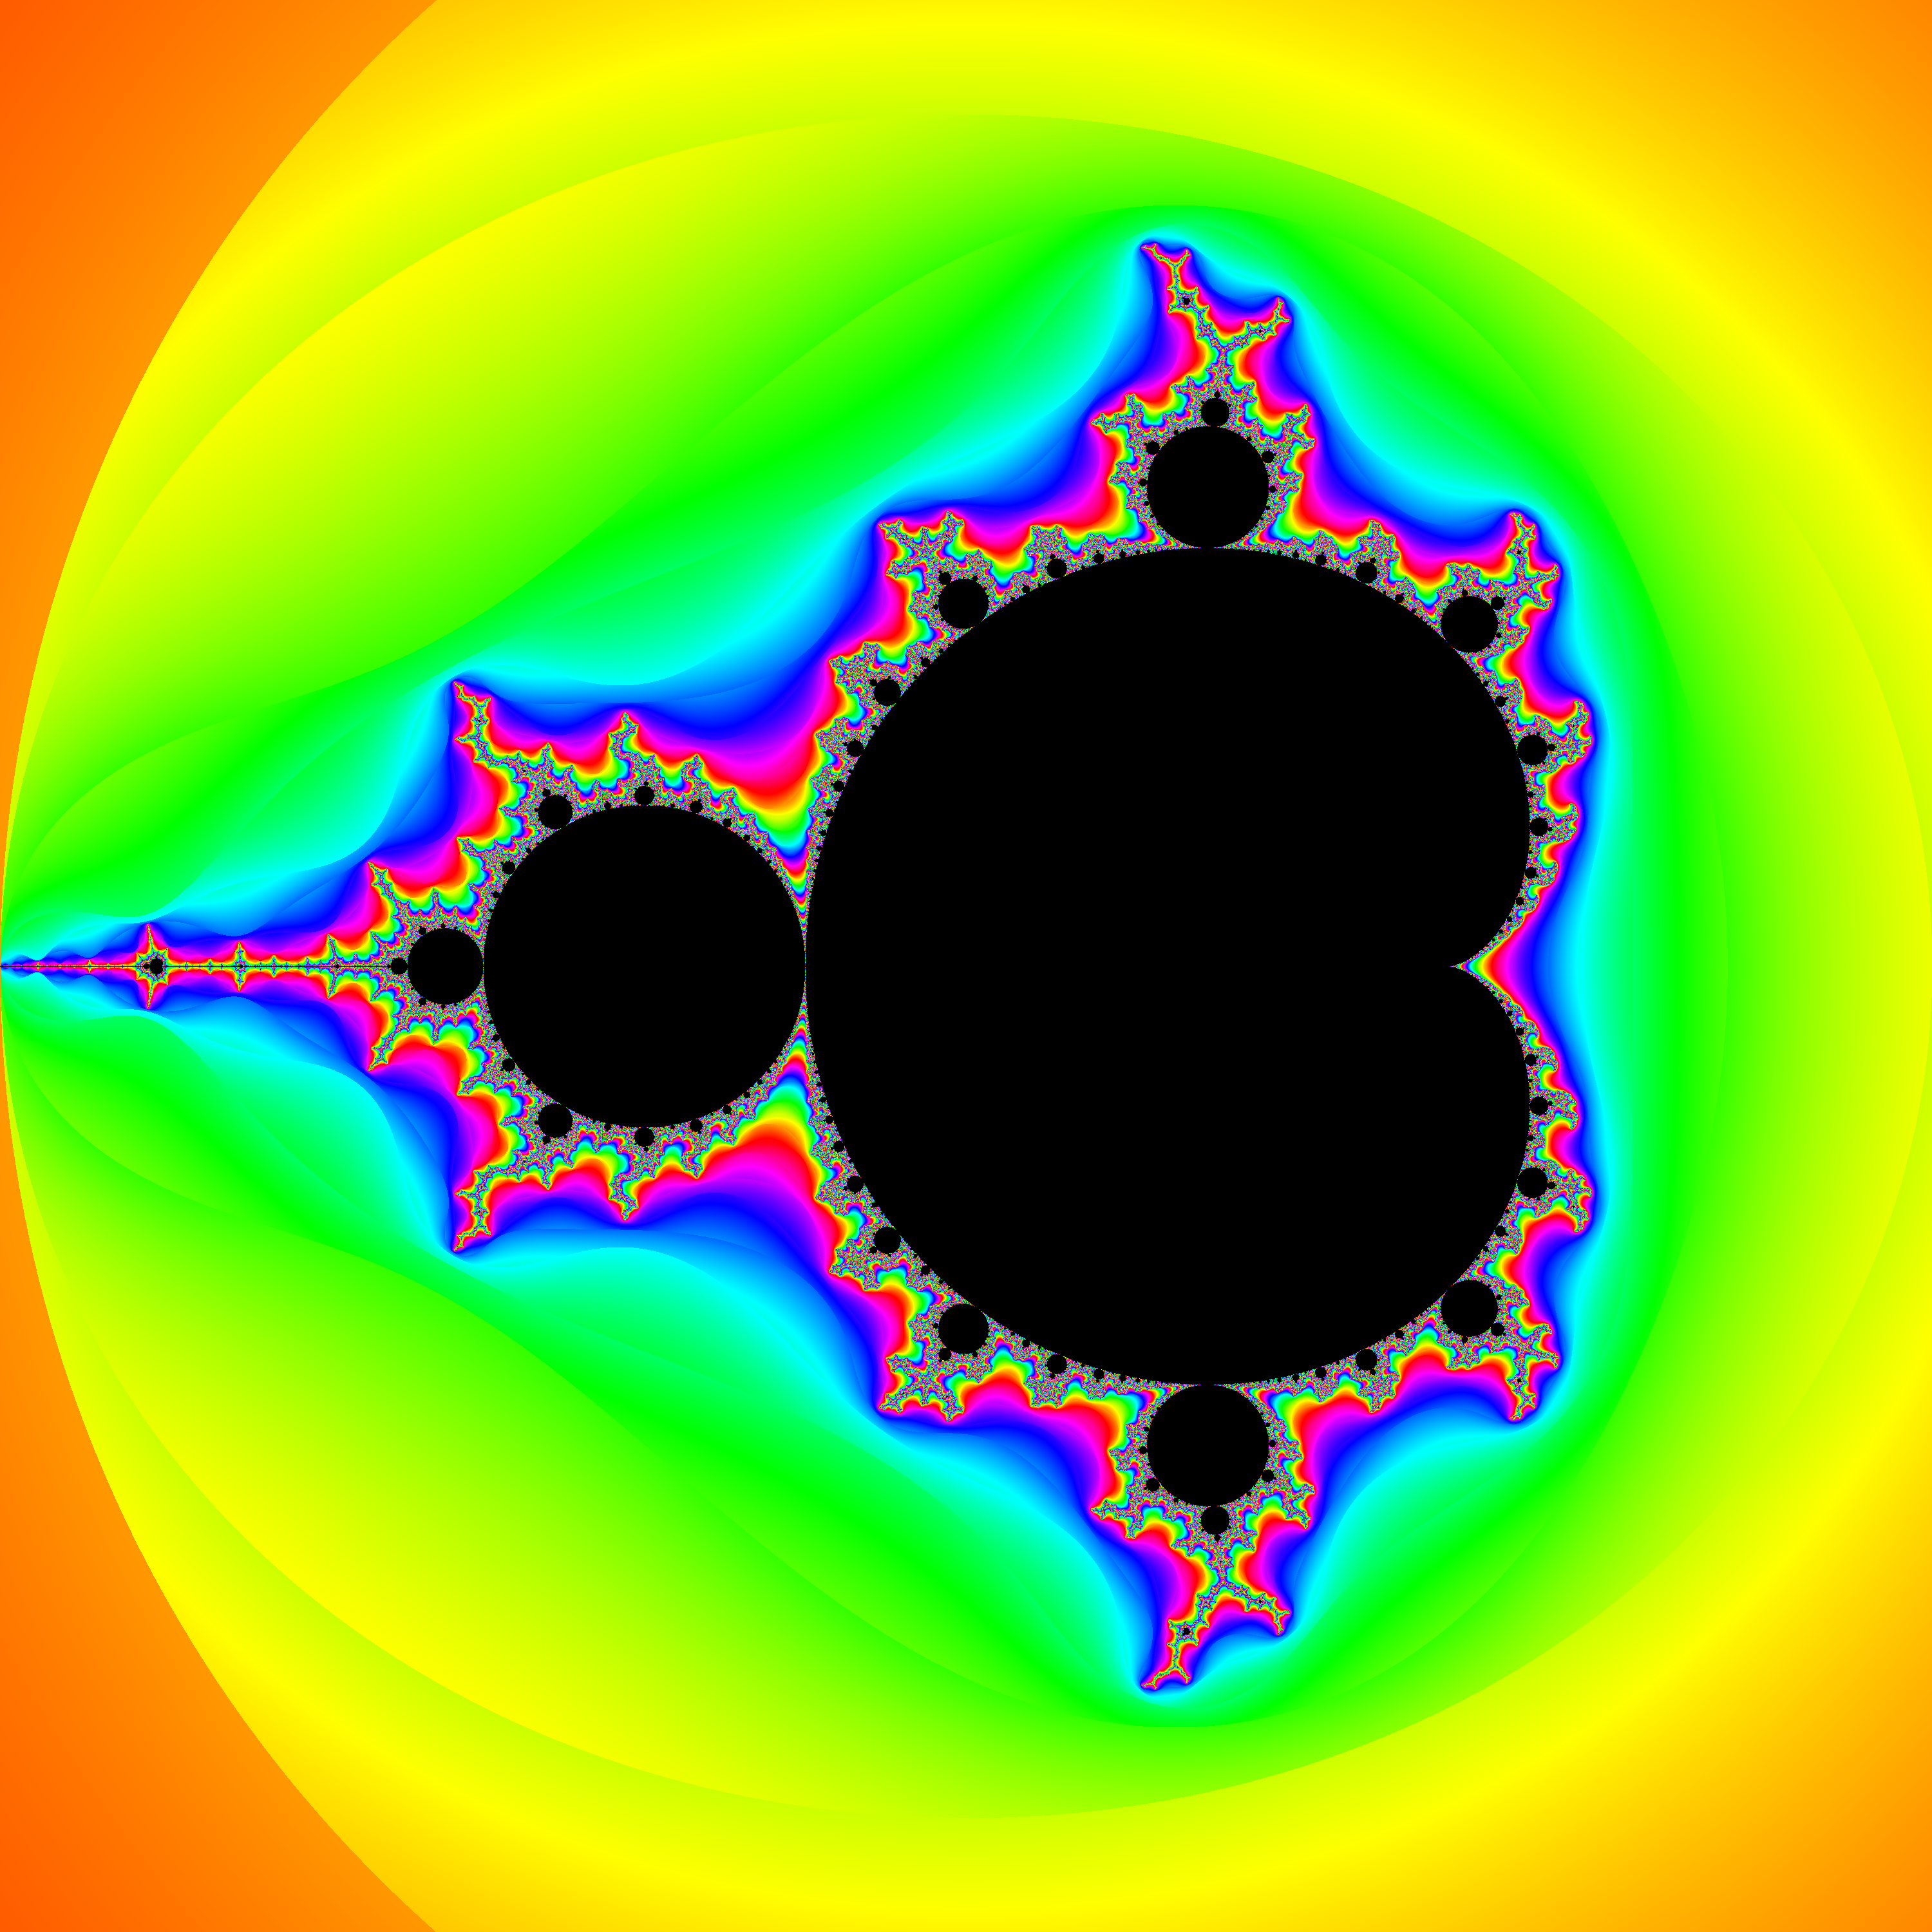
\includegraphics[width=0.95\textwidth]{gfx/figures/mandelbrot.png}
  \caption{Mandelbrot Set (generated by code of \ref{app:code:mandelbrot1})}
  \label{fig:methodology:mandelbrot}
\end{figure}
The Mandelbrot set is a famous subset of the complex numbers $\mathbb{C}$. Figure \ref{fig:methodology:mandelbrot} displays a coloriesed visualization of the set in the plane of complex numbers. To determine if a complex number $c$ is part of the Mandelbrot set, it is applied to the function \ref{equ:mandelbrot} with $z_{0}=0$.
\begin{equation}
  z_{n+1} = z_{n}^2 + c
  \label{equ:mandelbrot}
\end{equation}
If the value of $z_{n+1}$ does not diverge over n iterations, $c$ belongs to the Mandelbrot set. In Figure \ref{fig:methodology:mandelbrot}, all complex numbers $c$, for wich $z_{n+1}$ remains bounded over n iterations are colored black. All other $c$ are colored based on the number of iterations required for $z_{n+1}$ to diverge, with the color spectrum ranging from red (low iteration count) over to blue (high iteration count) indicating increasing iteration counts.

The calculation and visualization of the Mandelbrot set can be partitioned into multiple tasks. Each task executes the same source code but with different input parameters, which define a unique two-dimensional area in the complex plane. These tasks can be executed in parallel due to the independence of calculations between different areas. The implementation for this benchmark is provided in the Appendix. The source code for the native Go variant can be found in \ref{app:code:mandelbrot1} and its Go-to-WebAssembly counterpart in \ref{app:code:mandelbrot2}.